\documentclass[a4paper,11pt,titlepage]{article}

\usepackage{latexsym}
\usepackage{graphicx}
\usepackage{float}
\usepackage{url}
\usepackage{unicode}
\usepackage[polish]{babel}
\usepackage{titlesec}
\usepackage{listings}
\usepackage{xcolor}
\usepackage{setspace}
\usepackage{subfig}
\usepackage{tabularx}
\usepackage{courier}
\DeclareUnicodeCharacter{200B}{{\hskip 0pt}}

\definecolor{codeblue}{rgb}{0,0,0.6}
\definecolor{codegray}{rgb}{0.5,0.5,0.5}
\definecolor{codepurple}{rgb}{0.58,0,0.82}
\definecolor{backcolour}{rgb}{0.96,0.96,0.96}

\lstdefinestyle{code}{
    backgroundcolor=\color{backcolour},
    keywordstyle=\color{codeblue},
    numberstyle=\tiny\color{codegray},
    stringstyle=\color{codeblue},
    basicstyle=\ttfamily\footnotesize,
    breakatwhitespace=false,
    breaklines=true,
    captionpos=b,
    keepspaces=true,
    numbers=left,
    numbersep=5pt,
    showspaces=false,
    showstringspaces=false,
    showtabs=false,
    tabsize=2,
    basicstyle=\small
}

\lstset{style=code}

\newcommand{\sectionbreak}{\clearpage}
\author{Adam Talarczyk}
\title{Symulacje Monte Carlo}
\frenchspacing
\begin{document}
\begin{titlepage}
    \begin{center}

        \Huge
        \textbf{WYDZIAŁ NAUK ŚCISŁYCH I TECHNICZNYCH}

        \vspace{1.5cm}
        \LARGE
        Adam Talarczyk, Krystian Budulski, Mateusz Wrzoł
	\vspace{2cm}
	
	Symulacja Monte Carlo
	
	\vspace{5cm}
        \vfill

        \vspace{0.8cm}
	\Large
        Uniwersytet Śląski, Sosnowiec, 2021

    \end{center}
\end{titlepage}
\newpage

\tableofcontents
\newpage

\section{Zadanie 1}
Należy zmodyfikować kod dla aproksymacji stałej PI, aby sprawdzić jak rozmiar próbki wpływa na błąd aproksymacji. Błąd aproksymacji obliczamy jako wartość bezwględną różnicy, pomiędzy aproksymacją PI i wartością rzeczywistą PI (3.14159265). Należy przygotować wykres [Rysunek \ref{fig:wykres1}]

\begin{figure}[H]
\centering
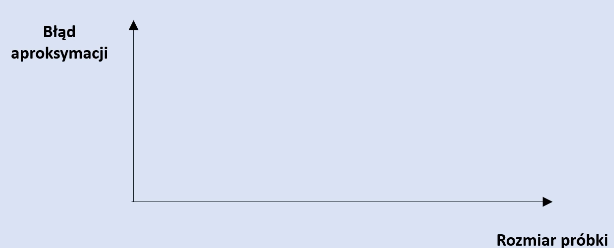
\includegraphics[width=1\columnwidth]{img/zad1.PNG}
\caption{Przykład wykresu}
\label{fig:wykres1}
\end{figure}

\subsection{Rozwiązanie}
Opis rozwiązania

\subsection{Kod źródłowy}
Listingi

\subsection{Wnioski}
Wnioski

\section{Zadanie 2}
Zaprogramować symulację Monte Carlo (np. w jęyku R), która pozwoli obliczyć pole powierzchni szarego obszaru, przedstawionego na poniższym rysunku [Rysunek \ref{fig:wykres2}]. Obliczyć błąd uzyskanego wyniku.

\begin{figure}[H]
\centering
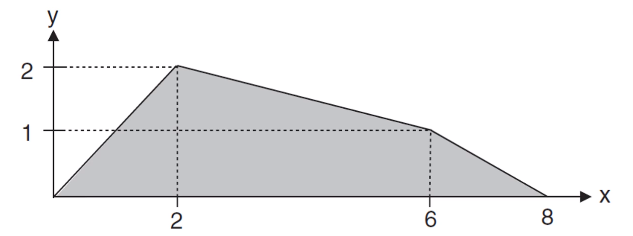
\includegraphics[width=1\columnwidth]{img/zad2.PNG}
\caption{Figura}
\label{fig:wykres2}
\end{figure}

\subsection{Rozwiązanie}
Opis rozwiązania

\subsection{Kod źródłowy}
Listingi

\subsection{Wnioski}
Wnioski

\end{document}
